\chapter{Methods}


\section{Noise approximation via STFT}

Limits of variance and stdev.

To better approximate the errors concerning white noise, a STFT is employed.

TODO: Comparison variance, standard deviation, mean noise. Scalability for other sensors.

Noise Tracking using DFT cite [Hen08]


\section{altitude comparison}

some mean ground has to be found to crossreference the various altitudes.

For standardization. The SI-unit meters is used for altitudes.

In the first draft. The altitude is sampled with 1Hz for computational speed and since gnss update rates are updated in a similar frequency.

\begin{figure}[h]
    \centering
    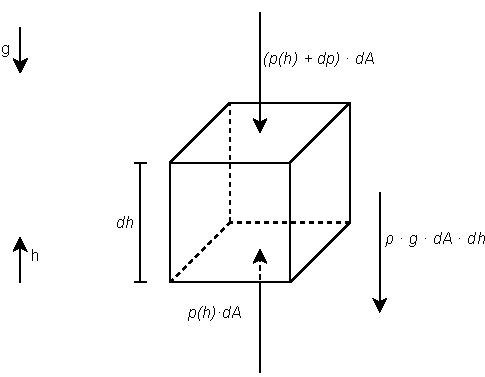
\includegraphics[width=.4\textwidth]{baro_dgl.drawio}
    \caption{Forces around a finitesimally small element}
    \label{fig:baro_FE}
\end{figure}

quick derivation of barometric formula based on the pressure pde.

\begin{equation}
    p=p_0 \cdot\left(1+\frac{a \cdot\left(h-h_0\right)}{T\left(h_0\right)}\right)^{\frac{-g}{a \cdot R}}
\end{equation}

\begin{conditions}
    p     & pressure at current altitude                     \\
    p_{0} & reference pressure\\
    h     & current altitude                                 \\
    h_{0} & reference altitude                                  \\
    a     & ISA Temperature Coefficient depending on altitude\\
    R     & 287Ideal Gas Constant
\end{conditions}

Resulting from the equilibrium around a finitesimally small element in figure \ref{fig:baro_FE}.

with for the volume:
$$dV = dA * dh$$

follows the force equilibrium for force terms as well as the gravity term $$m \cdot g$$


\begin{equation}
    0 = \rho \cdot g \cdot dA \cdot dh + ( p(h)- dp )\cdot dA - p(h) \cdot dA

    --> dp=-\rho\cdot g\cdot dh
\end{equation}

with ideal gas formula
$$p=ro*R*T$$

$$dp/p = -g/(R*T)*dh$$

and T = f(h) from Interational Standard Atmosphere ISA-correlation $$T=a*h + T_0$$ with a being defined as dT/dh and -6.5 K/km for the troposphere.

$$\frac{dp}{p}=\frac{-g}{R*(a*h+T_0)}*dh$$

integrating resolves in:
$$
ln(\frac{p}{p_0}) = - \frac{g}{a \cdot R} \cdot ln(\frac{a*h+T_0}{a*h_0+T_0})
$$
substituting:
\begin{conditions}
a &p/p_0\\
b & -g/a*R \\
c & (a*h+T_0)/(a*h_0+T_0) = 1+ (h-h_0)*a/(a*h_0+T_0)
\end{conditions}

with $$T(h_0) = a*h_0+T_0$$
--> $$c = 1+ (h-h_0)*a/T(h_0)$$


resolves in
$$ln(a) = b * ln(c) = ln(c^b) --> a = c^b$$

\begin{equation}
\frac{p}{p_0} = (1+\frac{a}{T(h_0)}*(h-h_0))^\frac{-g}{a*R}
\end{equation}


Also consider term for a=0

$$dp/p = -g/(R*T_0)*dh$$
ln(p/p_0) = -g/(R*T_0)*h
p/p_0= exp(-g/R*T_0)*h

solve towards c
$$c = a^(b^-1)$$

Resubstituting


$$
1+(h-h_0)*a/(T(h_0))=(p/p_0)^(1/(-g/(a*R))
$$
\begin{equation}
    h = (\frac{p}{p_0}^{\frac{-a*R}{g}}-1)*T(h_0)/a+h_0
    \caption{ISA-equation for altitude based on pressure differential}
\end{equation}

in aerospace context this gets used as follows.

$$p_0$$ is the reference pressure which gets used in conjunction with $$T_0$$.

Based upon reference pressure, the pressure value in at the boundary levels can be estimated.

Since Temperature is defined as follows:


\begin{table}[]
        \begin{tabular}{ccc}
            \toprule
            Geopotential Altitude [km] & Temperature T [K] & Temperature gradient a [K/km] \\ \midrule
            -2-0                       & 301.15            & -6.5                          \\
            0-11                       & 288.15            & -6.5                          \\
            11-20                      & 216.65            & 0                             \\
            20-32                      & 216.65            & 1                             \\
            32-47                      & 228.65            & 2.8                           \\
            47-51                      & 270.65            & 0                             \\
            51-71                      & 270.65            & -2.8                          \\
            71-80                      & 214.65            & -2                            \\ \bottomrule
        \end{tabular}
\caption{International Standard Atmosphere cite ISO75}
    \label{tab:isa_temp}
\end{table}


If altitude gets calculated, it needs to follow in two steps.
Based on ideal temperature at sea level

1. determine which ISA-Level is present by determining p/p_0 at the boundaries.
p/p_0 = f(h))


2. base calculation off of isa reference level
p/p

$$(a*h/T_0+1)/(a*h_0/T_0+1)$$

# TODO: implement g as a function of lat and long



For further use, the barometric formula will be expressed as  $$h = f(p,p_0)$$


\section{Finding a reference state}
Goal of this work is finding a reference frame for all parameters into which they can be transformed into and back.

A starting point which shall be considered is the geodetic reference.

it measures the aircraft's position by its displacement from the previously (ref?) discussed WGS84 system.

Meaning that altitude gets measured as the orthometric height (see ellipsoid height-geoid height).

Latitude and Longitude form the x and y axis of the COS. True heading forms the reference heading within the geodetic system.

All aircraft parameters related to motion and position of the aircraft should be attempted to be condensed into this form.